% !TEX root = ../../problems/hw01.tex
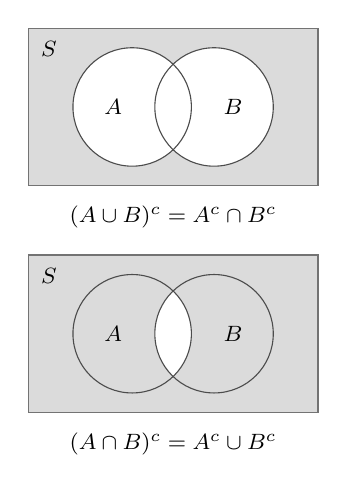
\begin{tikzpicture}[x=0.8cm,y=0.8cm,font=\footnotesize]
  \foreach \offset in {0,-3.6} {
    \begin{scope}[shift={(0,\offset)}]
      \fill[black!14] (0,0) rectangle (4.6,2.5);
    \end{scope}
  }
  % Removing both discs leaves the complement of their union.
  \fill[white] (1.65,1.25) circle[radius=0.94];
  \fill[white] (2.95,1.25) circle[radius=0.94];
  % Removing only the lens leaves the complement of the intersection.
  \begin{scope}[shift={(0,-3.6)}]
    \clip (1.65,1.25) circle[radius=0.94];
    \fill[white] (2.95,1.25) circle[radius=0.94];
  \end{scope}
  \foreach \offset in {0,-3.6} {
    \begin{scope}[shift={(0,\offset)}]
      \draw[black!55] (0,0) rectangle (4.6,2.5);
      \draw[black!70] (1.65,1.25) circle[radius=0.94];
      \draw[black!70] (2.95,1.25) circle[radius=0.94];
      \node at (1.35,1.25) {$A$};
      \node at (3.25,1.25) {$B$};
      \node[anchor=north west] at (0.05,2.45) {$S$};
    \end{scope}
  }
  \node at (2.3,-0.5) {$(A\cup B)^c=A^c\cap B^c$};
  \node at (2.3,-4.1) {$(A\cap B)^c=A^c\cup B^c$};
\end{tikzpicture}
